\chapter{System Design}
\label{ch:system_design}

\section{System Architecture}
\label{sec:system_architecture}

The system architecture is engineered as a modular, decoupled processing pipeline designed to isolate and quantify experimental randomness in machine learning workflows. Figure \ref{fig:sys_arch} illustrates the high-level architecture, encompassing five interconnected modules: Data Ingestion and Validation, Exploratory Data Analysis, Stratified Preprocessing, Multi-Seed Experimental Execution, and Stability Analytics.

\begin{figure}[H]
\centering
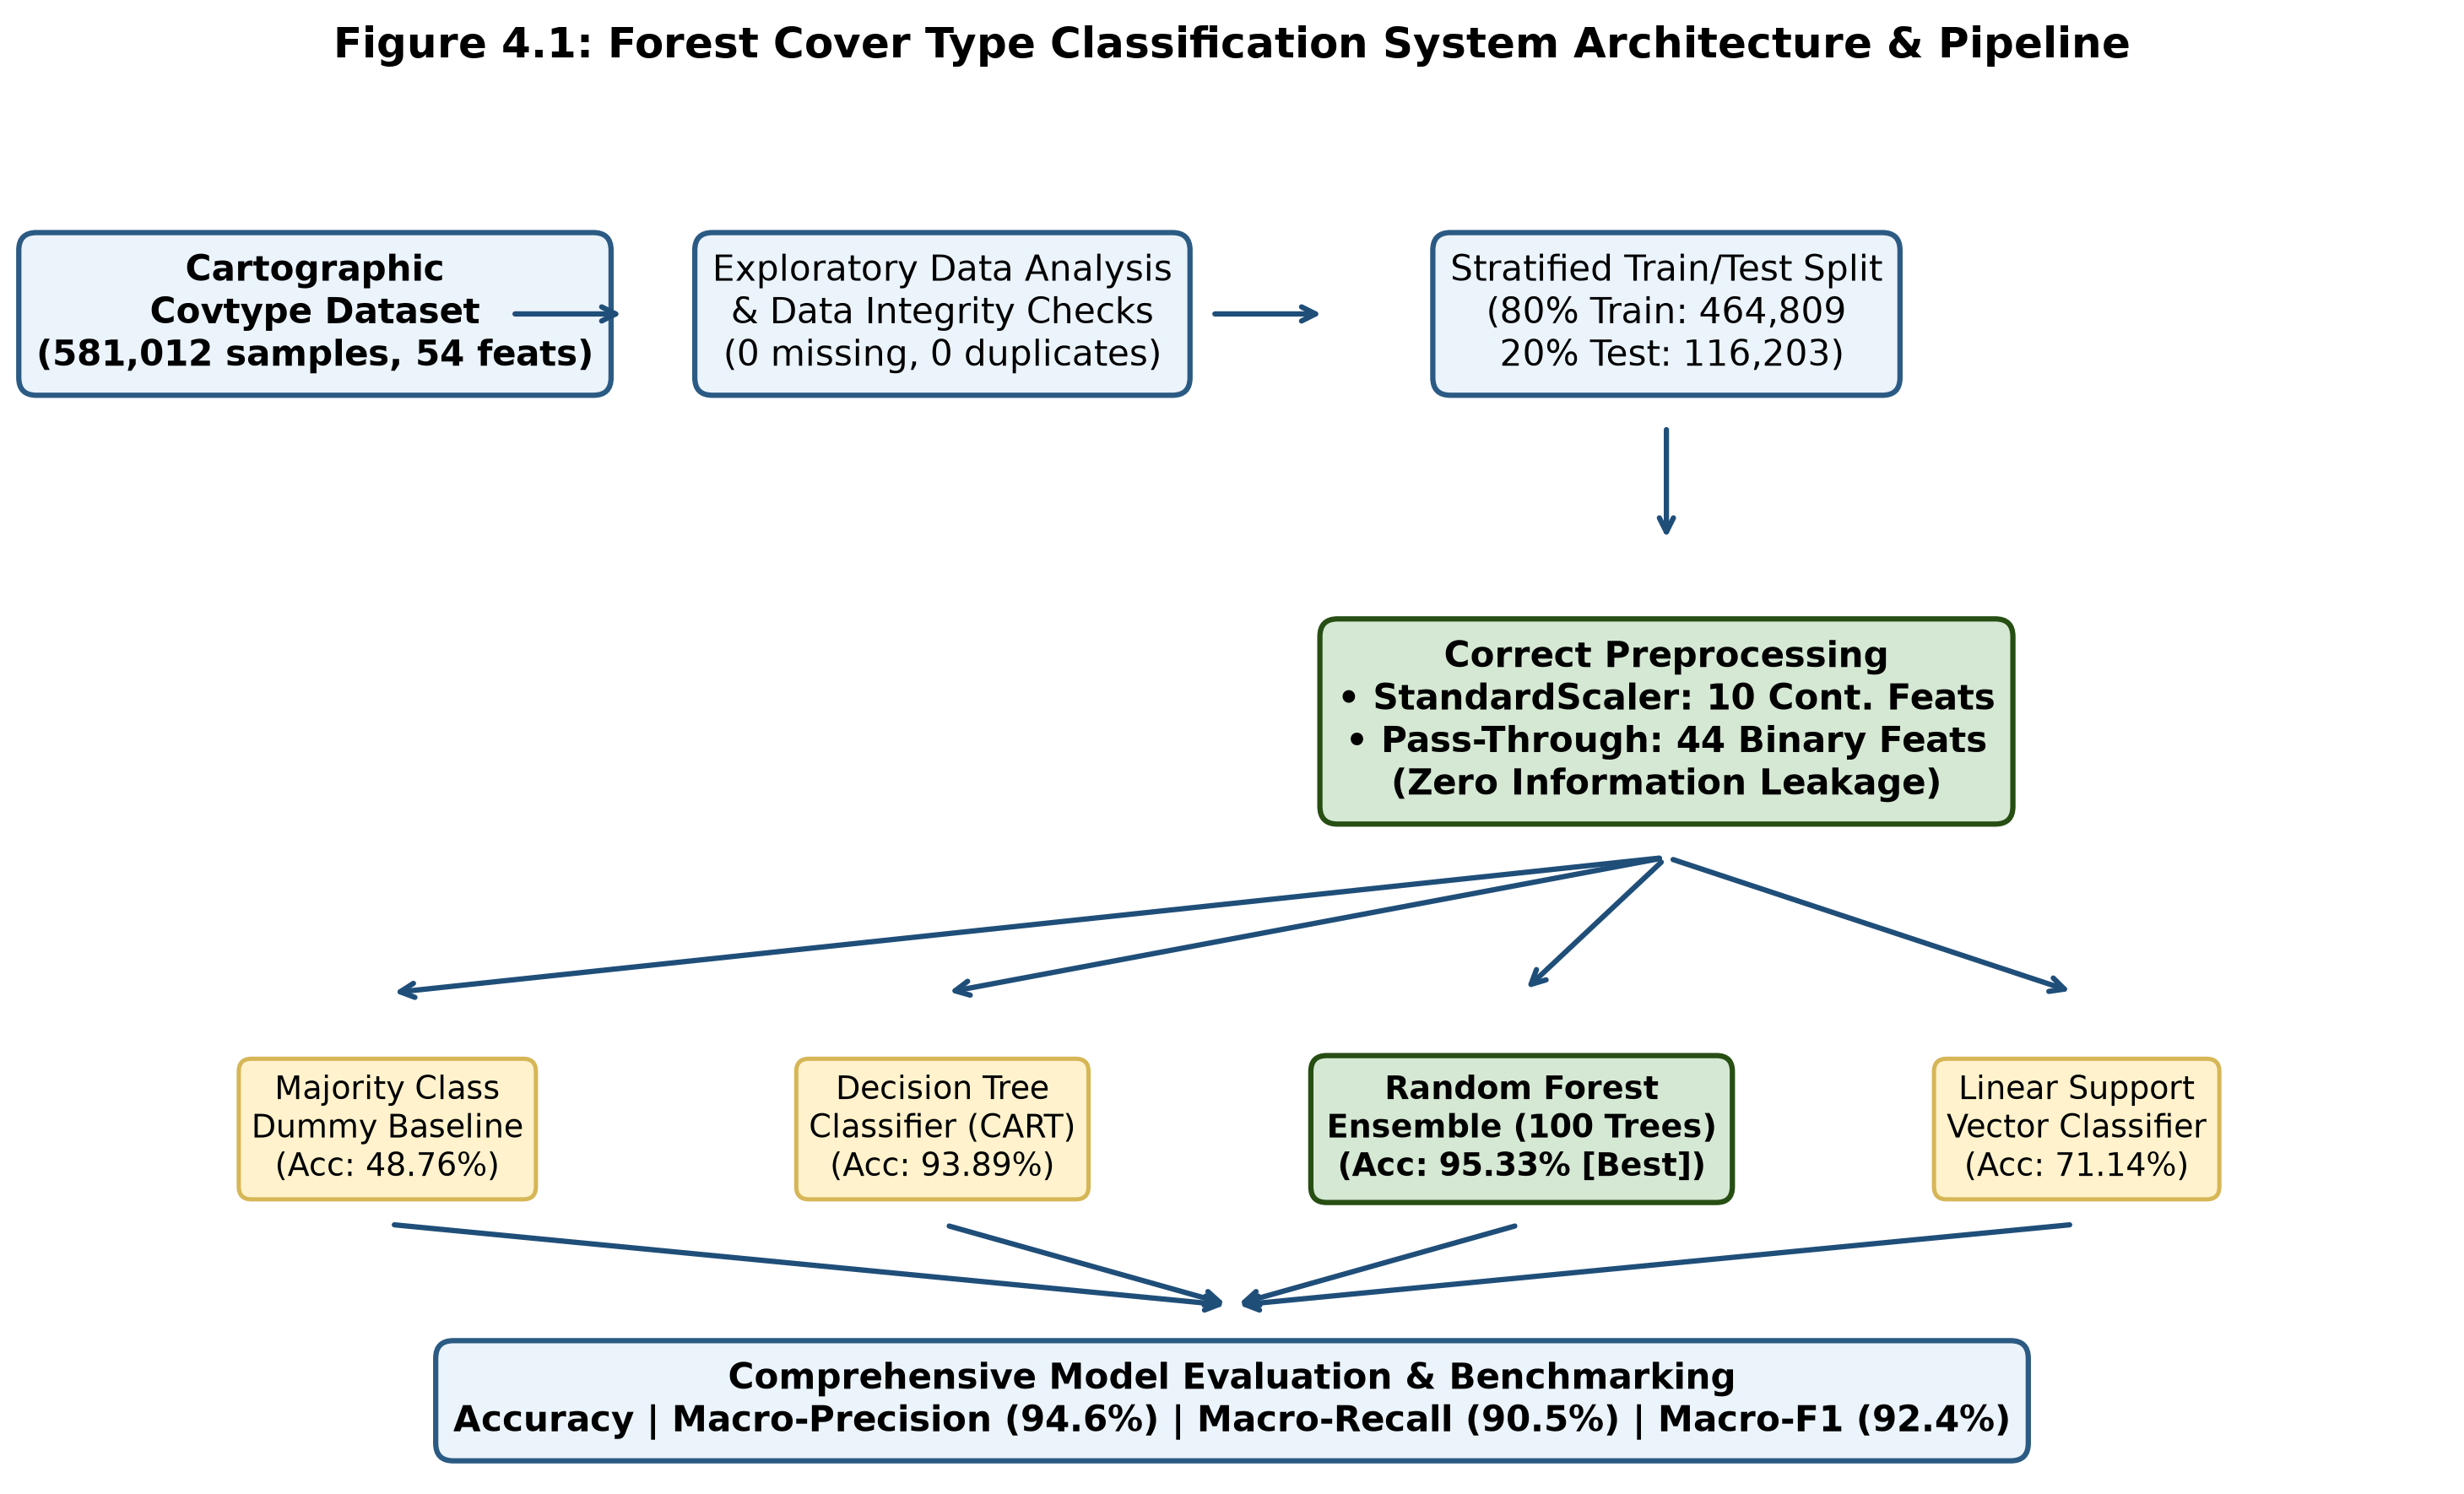
\includegraphics[width=0.92\textwidth]{figures/fig_system_architecture.png}
\caption{End-to-End System Architecture for Machine Learning Randomness and Stability Analysis}
\label{fig:sys_arch}
\end{figure}

The pipeline executes deterministically through explicitly managed random seeds, ensuring that intermediate artifacts (subsampled frames, scaled tensors, and split indices) remain strictly reproducible across computational runs.

\section{System Workflow and Use Case Modeling}
\label{sec:system_workflow}

The operational workflow follows a strict, sequential experimental lifecycle designed to guarantee reproducibility, modular evaluation, and rigorous empirical validation:
\begin{enumerate}
    \item \textbf{Ingestion Trigger:} The pipeline loads the full Forest CoverType dataset (581,012 records across 54 cartographic, wilderness, and soil features) from the repository.
    \item \textbf{Exploratory Profiling:} Data distributions, continuous feature skews, multi-collinearity, and class imbalances across all 7 cover types are comprehensively profiled.
    \item \textbf{Stratified Sampling:} A class-balanced 10,000-instance subsample is extracted using a fixed random seed (\texttt{random\_state=42}) to preserve exact population class proportions.
    \item \textbf{Phase 1 Baseline Benchmark:} Baseline models (Decision Tree, Random Forest, Linear SVM) are trained on a standardized 80/20 train-test partition with baseline seed $S_0=42$.
    \item \textbf{Phase 2 Split-Seed Sensitivity Assessment:} The data partitioner systematically iterates over five distinct random seeds ($\mathcal{S}_{\text{split}} = \{0, 1, 42, 99, 123\}$). For each partition, preprocessing scalers are fitted strictly on the training partition, models are trained from scratch, and test accuracy and Macro-F1 are logged to measure stochastic sensitivity.
    \item \textbf{Phase 3 Cross-Validation \& Dispersion Analysis:} 5-fold stratified cross-validation is evaluated across three distinct shuffle seeds ($\mathcal{S}_{\text{cv}} = \{11, 22, 33\}$), computing mean accuracy and standard deviation error bars across folds.
    \item \textbf{Phase 4 Training Dataset Size Scaling:} The sample volume is dynamically scaled across $N_{\text{train}} \in \{2000, 5000, 8000\}$ samples to assess asymptotic learning trajectories and minority class Macro-F1 dynamics.
    \item \textbf{Phase 5 Hyperparameter Capacity Tuning:} Model capacity and regularization trade-offs are analyzed by sweeping Decision Tree maximum depth ($d \in \{5, 10, \text{None}\}$) and Random Forest ensemble tree counts ($B \in \{50, 100, 200\}$).
    \item \textbf{Phase 6 Feature Group Ablation:} The discriminative power of the 10 continuous terrain features is evaluated in isolation and compared against the full 54-feature set to assess dimensional efficiency.
    \item \textbf{Phase 7 Bitwise Reproducibility Audit:} Duplicate back-to-back training runs are executed under identical seed configurations to perform strict bitwise verification checks ($\hat{\mathbf{y}}_1 == \hat{\mathbf{y}}_2$).
    \item \textbf{Phase 8 Reporting \& Diagnostic Visualization:} Publication-grade metric tables, error bar charts, sensitivity histograms, and performance trade-off curves are compiled and rendered.
\end{enumerate}

\begin{figure}[H]
\centering
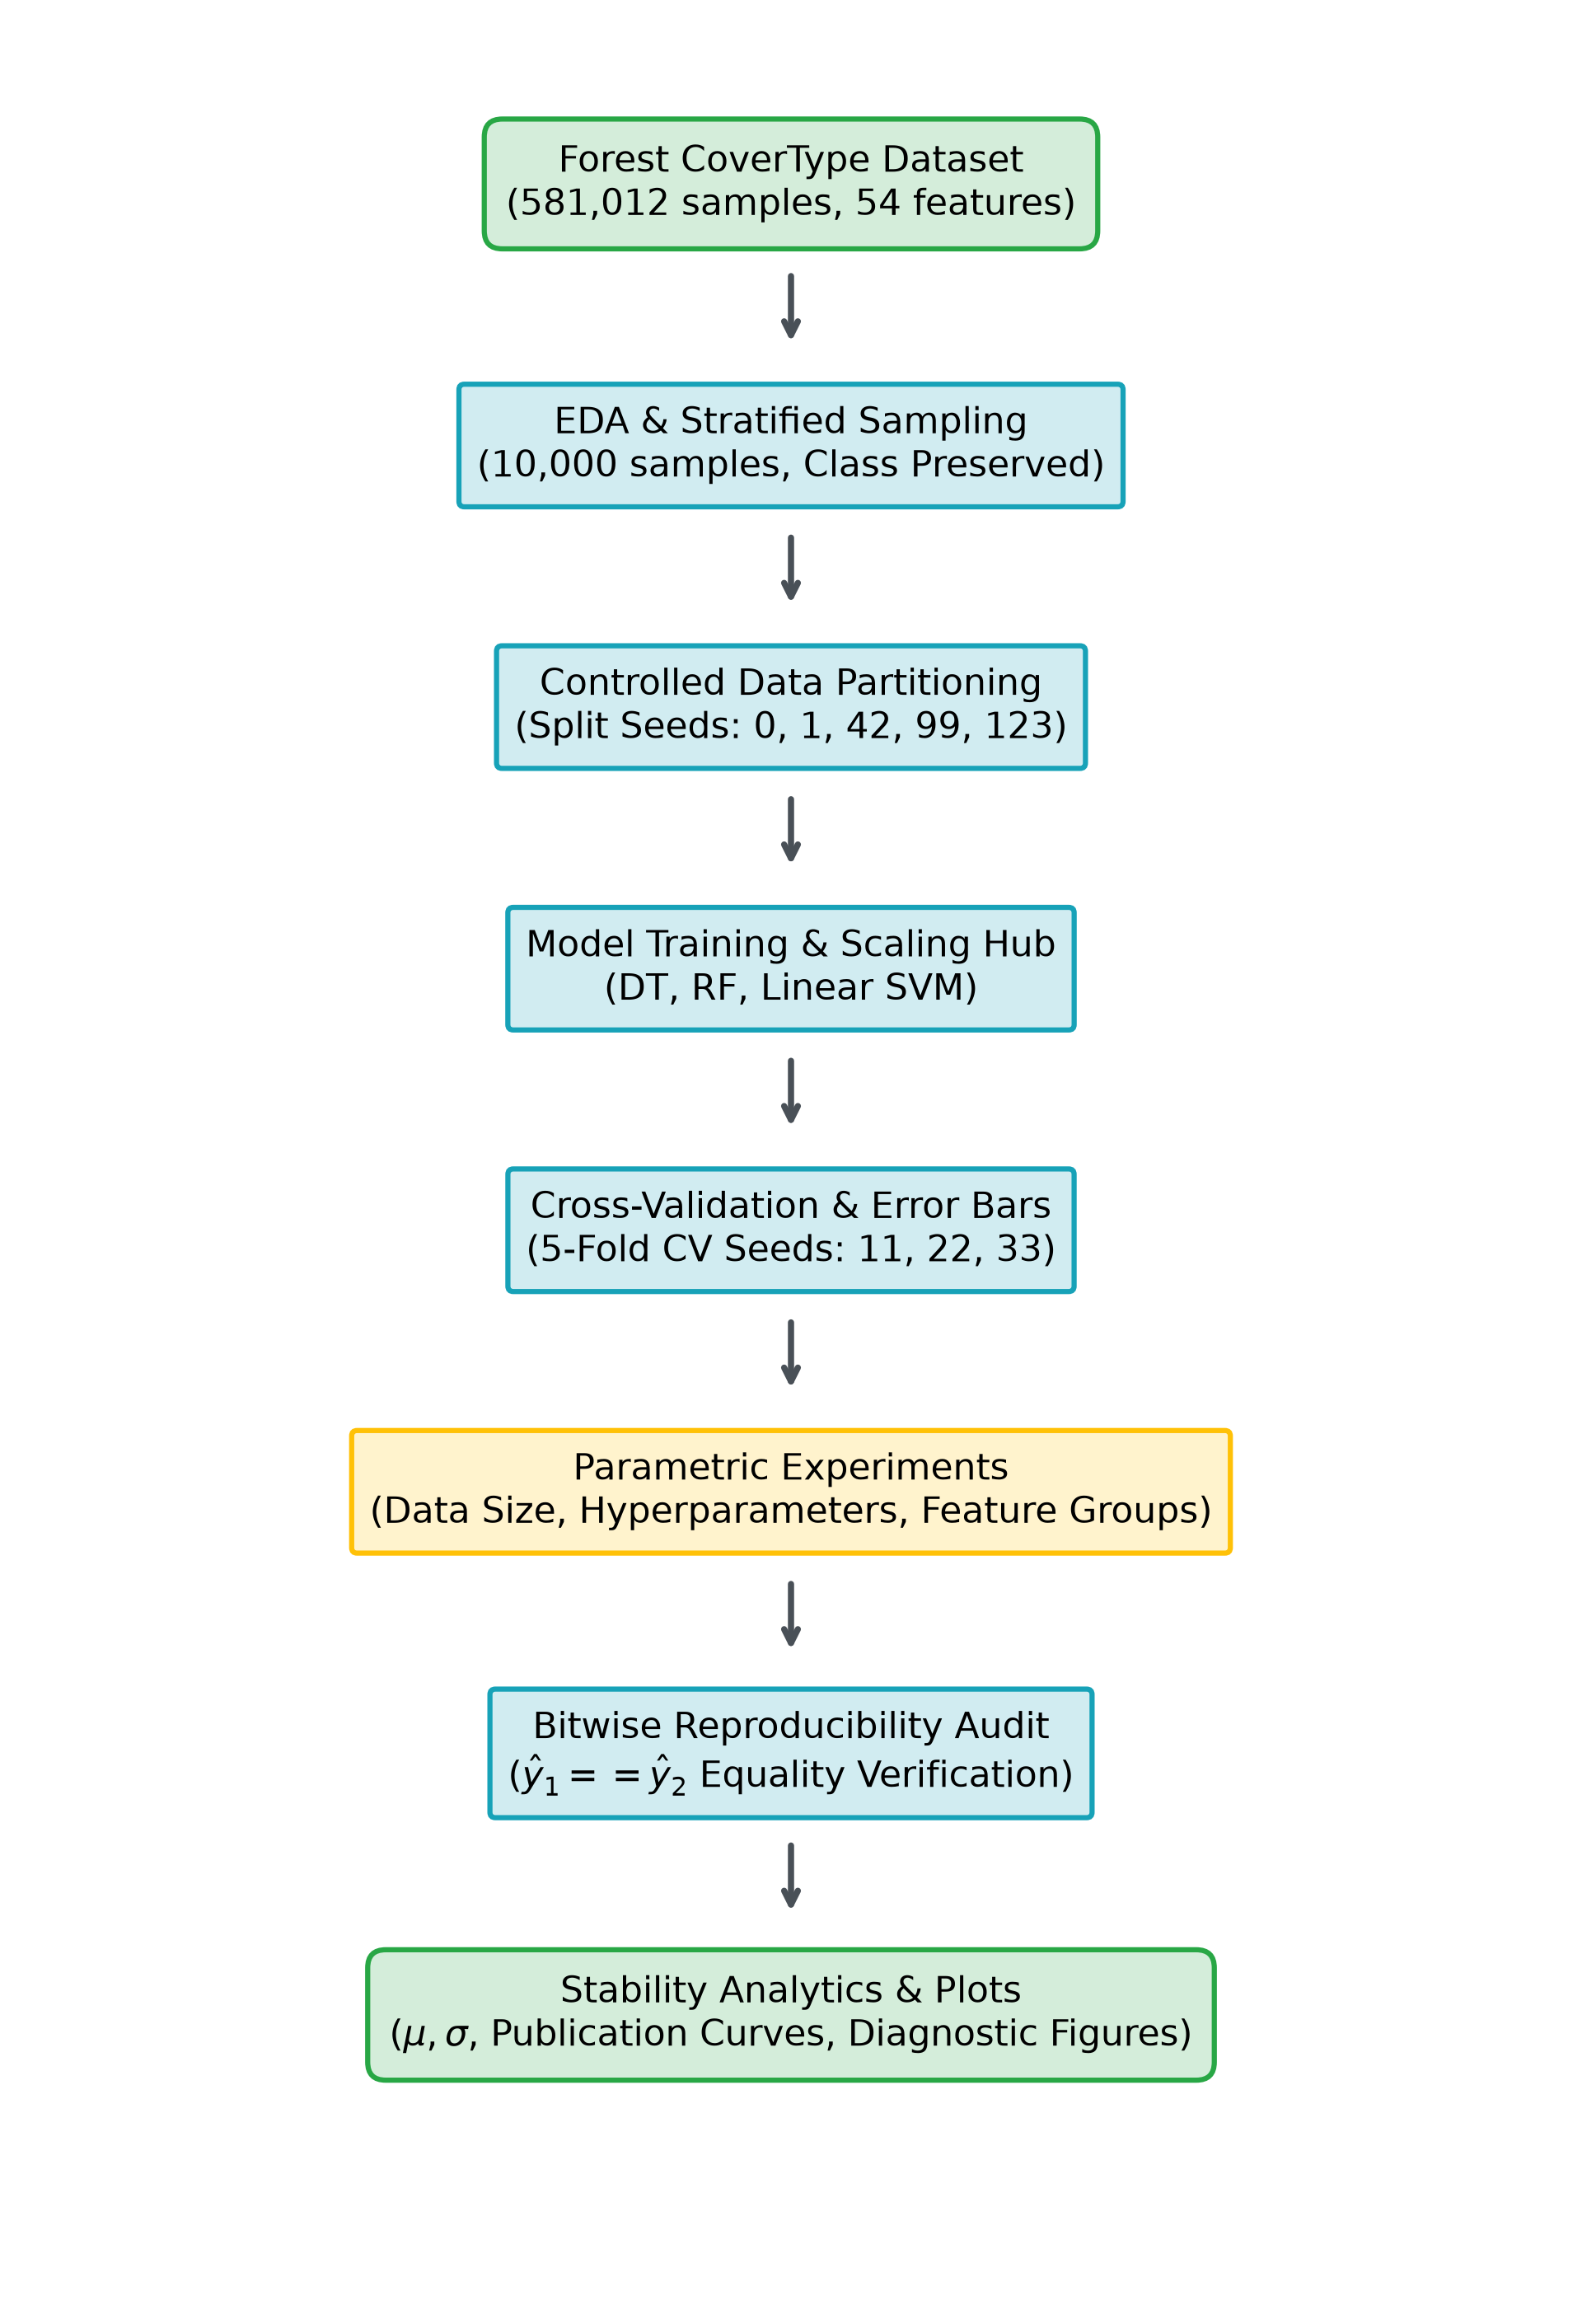
\includegraphics[width=0.72\textwidth]{figures/fig_system_workflow_diagram.png}
\caption{Comprehensive End-to-End System Workflow Pipeline Diagram}
\label{fig:workflow_flowchart}
\end{figure}

\section{Data Flow Modeling}
\label{sec:data_flow}

Data flow within the system is modeled across two hierarchical levels:

\subsection{Level 0 Data Flow (Context Diagram)}
At the context level, external input consists of the raw Forest CoverType data and user-defined seed arrays. The system processes these inputs and produces stability metrics, performance tables, and diagnostic plots.

\subsection{Level 1 Data Flow (Decomposed Processes)}
At Level 1, the transformation flow is partitioned into five distinct computational stages:
\begin{itemize}
    \item \textbf{Process 1.0 (Data Stratifier):} Consumes the full dataset and outputs the class-balanced 10,000-sample dataset $\mathcal{D}_{\text{sub}}$.
    \item \textbf{Process 2.0 (Train-Test Splitter):} Accepts $\mathcal{D}_{\text{sub}}$ and split seed $s \in \mathcal{S}_{\text{split}}$, generating paired splits $(\mathbf{X}_{\text{train}}^s, \mathbf{y}_{\text{train}}^s)$ and $(\mathbf{X}_{\text{test}}^s, \mathbf{y}_{\text{test}}^s)$.
    \item \textbf{Process 3.0 (Preprocessing Engine):} Fits \texttt{StandardScaler} strictly on continuous columns of $\mathbf{X}_{\text{train}}^s$, transforms continuous columns in both sets, and concatenates normalized columns with untouched binary features.
    \item \textbf{Process 4.0 (Model Execution Engine):} Trains Decision Tree, Random Forest, and Linear SVM models and computes predictions $\hat{\mathbf{y}}^s$.
    \item \textbf{Process 5.0 (Metric Aggregator):} Gathers point metrics across all seeds, computing statistical distributions ($\mu, \sigma$), cross-validation summaries, and bitwise verification flags.
\end{itemize}

\section{Module Description}
\label{sec:module_description}

The system comprises five core software modules:

\paragraph{Module 1: Ingestion and Stratified Sampler}
Interfaces with \texttt{sklearn.datasets.fetch\_covtype} to load feature matrices and target arrays. Handles initial type verification and executes stratified sampling using \texttt{StratifiedShuffleSplit} to guarantee identical class distributions between the sample and the population.

\paragraph{Module 2: Feature Transformation Engine}
Maintains strict segregation between continuous cartographic features ($p_{\text{cont}} = 10$) and binary soil/wilderness indicators ($p_{\text{bin}} = 44$). Implements \texttt{StandardScaler} normalization exclusively on training continuous features to guarantee zero information leakage.

\paragraph{Module 3: Baseline Classifier Hub}
Encapsulates model initialization, hyperparameter assignment, and baseline fitting using a standardized seed ($S_0 = 42$). Generates classification reports, confusion matrices, and multi-class F1 benchmarks.

\paragraph{Module 4: Split-Seed Sensitivity Harness}
Orchestrates systematic multi-seed iterations across seed values $\{0, 1, 42, 99, 123\}$. Records metrics into structured pandas DataFrames, enabling variance quantification and comparative distribution profiling.

\paragraph{Module 5: Cross-Validation \& Reproducibility Auditor}
Executes $5$-fold stratified cross-validation across three distinct shuffle seeds $\{11, 22, 33\}$. Furthermore, executes duplicate training runs with identical seed parameters and computes bitwise equality checks across prediction arrays ($\hat{\mathbf{y}}_1 == \hat{\mathbf{y}}_2$).

\section{Summary}
\label{sec:design_summary}

The system design establishes a clean, decoupled architecture that isolates stochastic variables while enforcing strict experimental hygiene. The modular structure guarantees that all preprocessing, training, and evaluation steps operate deterministically. The implementation of this architecture is presented in Chapter \ref{ch:implementation}.
